\documentclass[a4paper]{article}

%% Language and font encodings
\usepackage[english]{babel}
\usepackage[utf8x]{inputenc}
\usepackage[T1]{fontenc}
\usepackage{authblk}
\usepackage[usenames, dvipsnames]{color}
\usepackage[table]{xcolor}
%% Sets page size and margins
\usepackage[a4paper,top=2cm,bottom=2.4cm,left = 2 cm, right =2cm]{geometry}

%% Useful packages
\usepackage{amsmath}
\usepackage{amssymb}
\usepackage{graphicx}
\usepackage[colorinlistoftodos]{todonotes}
\usepackage[colorlinks=true, allcolors=blue]{hyperref}

\renewcommand*\familydefault{\sfdefault}
\usepackage[scaled = 0.92]{helvet}


%% define
\definecolor{odd_row}{RGB}{250,250,250}
\definecolor{even_row}{RGB}{217,217,217 }
\definecolor{header}{RGB}{197,197,197 }
\definecolor{footer}{RGB}{57,57,57 }
\font\titlefont=cmr9 at 30pt

%% define header and footer
\usepackage{fancyhdr}
\pagestyle{fancy}
\renewcommand{\headrulewidth}{0.4pt}
\renewcommand{\footrulewidth}{0.4pt}
\lhead{qplum Investment Research}
\rhead{
\includegraphics[width=2cm]{qplum_logo.png}}
\cfoot{\color{footer}\footnotesize
\normalsize\thepage
}


\author[1]{Ankit Awasthi\thanks{ankit.awasthi@circulumvite.com}}
\author[1]{Vinit Darda\thanks{vinit.darda@tworoads.co.in}}
\author[1]{Gaurav Chakravorty \thanks{gchak@qplum.co}}

\affil[1]{qplum Investment Research}

\title{How to make high-frequency-trading models that maximize PnL instead of r-squared}
\date{}


\begin{document}

\maketitle

\begin{abstract}
Most of the firms engaged in trading at a high frequency, a.k.a. the high-frequency-trading industry, try to predict the price of the traded security some time interval in future. However, a higher accuracy in price prediction does not always translate to higher profits. Profitability is the real metric that the portfolio manager cares about. In this paper, we will talk about the history of price prediction and why profit-maximization has had little success so far. We will then document our efforts to shift from price prediction models to profit maximization based trading model optimization techniques. We will give a blueprint for high frequency trading firms trying to make a similar transition towards pnl based modeling.
\end{abstract}


\section{Motivation}
Most high frequency trading \(HFT\) firms use a short-term price prediction model. This effort at price prediction has been dominated by linear regression models. More recently people have started using more sophisticated models, without deviating from the paradigm of future price prediction. More sophisticated modeling techniques tend to have a higher number of parameters and hence greater degrees of freedom. There are legitimate concerns of over-fitting with more sophisticated models. However, regardless of the complexity of the modeling technique that is being used, there is a general effort towards making the model more relevant.\\
There are two problems HFT firms face when using price prediction models: 
\begin{itemize}
	\item A higher accuracy in price prediction, even on the day that we are trading with a model, does not always translate to higher profits.
	\item We don't want to overfit to past data. We care about future investing gains and not the returns we would have attained in the past, when investing in a strategy. \cite{Saruchi2016}
\end{itemize}

Price prediction is an intuitive way to optimize models when we are expecting to hold on to the position for a long duration. In such situations the profits and losses of the trading would be dominated by price at the time. However in the HFT industry, the execution aspects of the trade and short term market microstructure aspects affect the trading profits a lot more than price prediction. During the heyday of the HFT industry, firms had been known to ignore the model altogether in an effort to get to the top of the queue and buy and sell for profit even without the price moving much. Today, however, we see a substantial slowing down of the HFT industry. Trading horizons are now significantly longer than before and prices can change appreciably in the time it takes for HFT firms to get out of the trade. In many ways making better models has become a lot more important.

\section{Overview of algo-trading strategy development and
  optimization}
\label{sec:overview}
work in progress

\section{Pnl based modeling from scratch}
\label{sec:ankit-work1}
This work was motivated by experiments conducted by Ankit and Rakesh
where they observed that trading with models with high correlation did
not lead to higher trading profits. They tried to change the hill
climb based subset selection approach from an objective function that
would maximize r-squared to an obective function that would maximize
profits.\\
Observation that the search rocess would stop more often than not with
four to five indicators.\\
Observations that we would often see very poor performance in out of
sample data. I am not sure if we ever tried trading with the few
models that would still have decent performsnce in pout of sample
data.\\
One of the problems we faced was that when we tried to add one
indicator to an empty model and do a hillclimb based searching for an
optimal model, often the results of an empty model that had a low
trading horizon \(TTC\), was very negative. Thus an immediate
improvement could be made by selecting indicators that in essence
inhibioted tarding. However that was not the aim of the exercise.
\section{Constrained search of a model that maximizes profits}
\label{sec:ankit-work2}
Here we tried to stay away from syubset selection, and we would only
try to learn the weights from scratch. The hope was that now, that we
are not trying to figure out which five indicators to select from a
set of hundred, we might be overfitting less.

\section{Adding and removing one indicator to the model}
\label{sec:aim}
Since we had a problem in the previosu effort of starting with an
empty model as a baseline, here we tried to start with an existing
model. This original model that we would start with, was probably generated by a penalized linear
regression method like ridge regression or lasso, and more often than
ot it was chosen because it had demonstrated decent reseults in PnL
space. This was a much more comfortable starting point, for a PnL
based search, and we were unlikely to land into situations where not
trading would be more optimal than the current model. We will carry
forward this intuition in section \ref{sec:optimal-set}.

\section{Find a better model by perturbing weights of an existing
  model}
\label{sec:fbmfs}
Like the section \ref{sec:aim} here, we would start with an existing
model and we would try to perturb the weights in an effort to arrive
at a model that had better profits on the given trading days. Since
the search space is larger than what we were doing in section \ref{sec:aim}

\section{Moving to pnl-space linear combination}
\label{sec:vinit-work}
work in progress

\section{Finding a set of models instead of one optimal model}
\label{sec:optimal-set}
The assumption here is that there is a natural seasonality in
markets. The prevalent trade changes. Finding one model that does well
in all markets is an inherently tougher problem. What might be much
easier is to figure out a small set of ``representative'' models, and
perhaps later, model-paramset combinations i.e. ``strategies'' such
that at least one of these models performs very well on the given
trading days. We are optimizing the sum of profits of the set of
models, where we have the luxury of choosing the model with the
greatest profits every day. The reason we are looking at the best
model is not a hope to overfit but that we see that model as a high
level expression of the nature of the day. We are using this small set
of models to ``describe'' that trading day. The question now is how to
find this set of models and what do we do when we have found this set
of models. Let's assume also that we have been told the number, say $N_S$ of
models that can be in this set.

\subsection{How to find a good set of models that describe a given set
  of trading days}
\label{subsec:optimal-set-finding}
We will borrow ideas from collaborative filtering \cite{Koren2009}
\cite{Ruslan2007rbmnetflix} \cite{ZhouWilkinsonnetflix} and section
\ref{sec:vinit-work}. Starting with a baseline equal weight model for all
the indicators, we will use some way of perturbing these and searching
far and wide from the original point. We will try to come with a small
set of perturbed strategies, say around fifty. Now we will try to
backtest these fifty strategies on the given set of trading
days. 

As the Netflix Prize has demonstrated, matrix factorization models are 
superior to classic nearest-neighbor techniques for producing recommendations, 
allowing the incorporation of additional information such as implicit 
feedback, temporal effects and confidence levels.

The traditional approach to recommendation of strategies 
is not very dissimilar to recommendation of products in 
ecommerce websites. It is similar to what is called the 
``content-filtering approach''. It involves finding external 
features to build a ``profile'' for each product, or in our 
case, strategy. An alternative to content filtering does not 
require experts to find features to describe each option. 
The latent-factor approach of collaborative filtering is 
what we are working on here. Let's see the math.

Suppose we have $nD$ trading days and if we were to generate $nS =
50$ strategy configs, we would be able to compute an $nS X nD$ 
matrix of pnl changes. Let's call this results matrix $R$. 
Then we could factorize this matrix into an $nS X k$ matrix $S(k)$ 
and a $k X nD$ matrix $D(k)$ such that $R \approx S(k) * D(k)$. 
Here we are trying to find $k$ latent factors that describe 
each trading day and similalry $k$ latent factors that describe 
each strategy.
We can think of each row in $S(k)$ as a k-dimensional footprint of every
strategy. $S(k)[i:]$ or the $i^{th}$ row in the matrix $S(k)$ denotes
the vector describing the $i^{th}$ strategy in terms of latent
factors. $D(k)^T[j:]$ or the $j^{th}$ column of $D(k)$ denotes the
vector describing the $j^{th}$ day in terms of latent factors.

Currently we are assuming that the measurement of profits can
only be done at the granularity of the trading day. We believe that
the analysis lends itself equally to hourly or fifteen-minute PNL
changes as well.

We had faced two problems in the ``What Kind of a Day is it?''
i.e. ``WKoDii'' project. The factors that we were coming up with often
did not separate the good strategies from bad strategies in our
pool. The second problem was that the process of coming up with
factors and the infrastructure around it was becoming more and more
subjective. It was turning into an art like feature engineering on its
own.

\begin{centering}
	\begin{figure}
		
		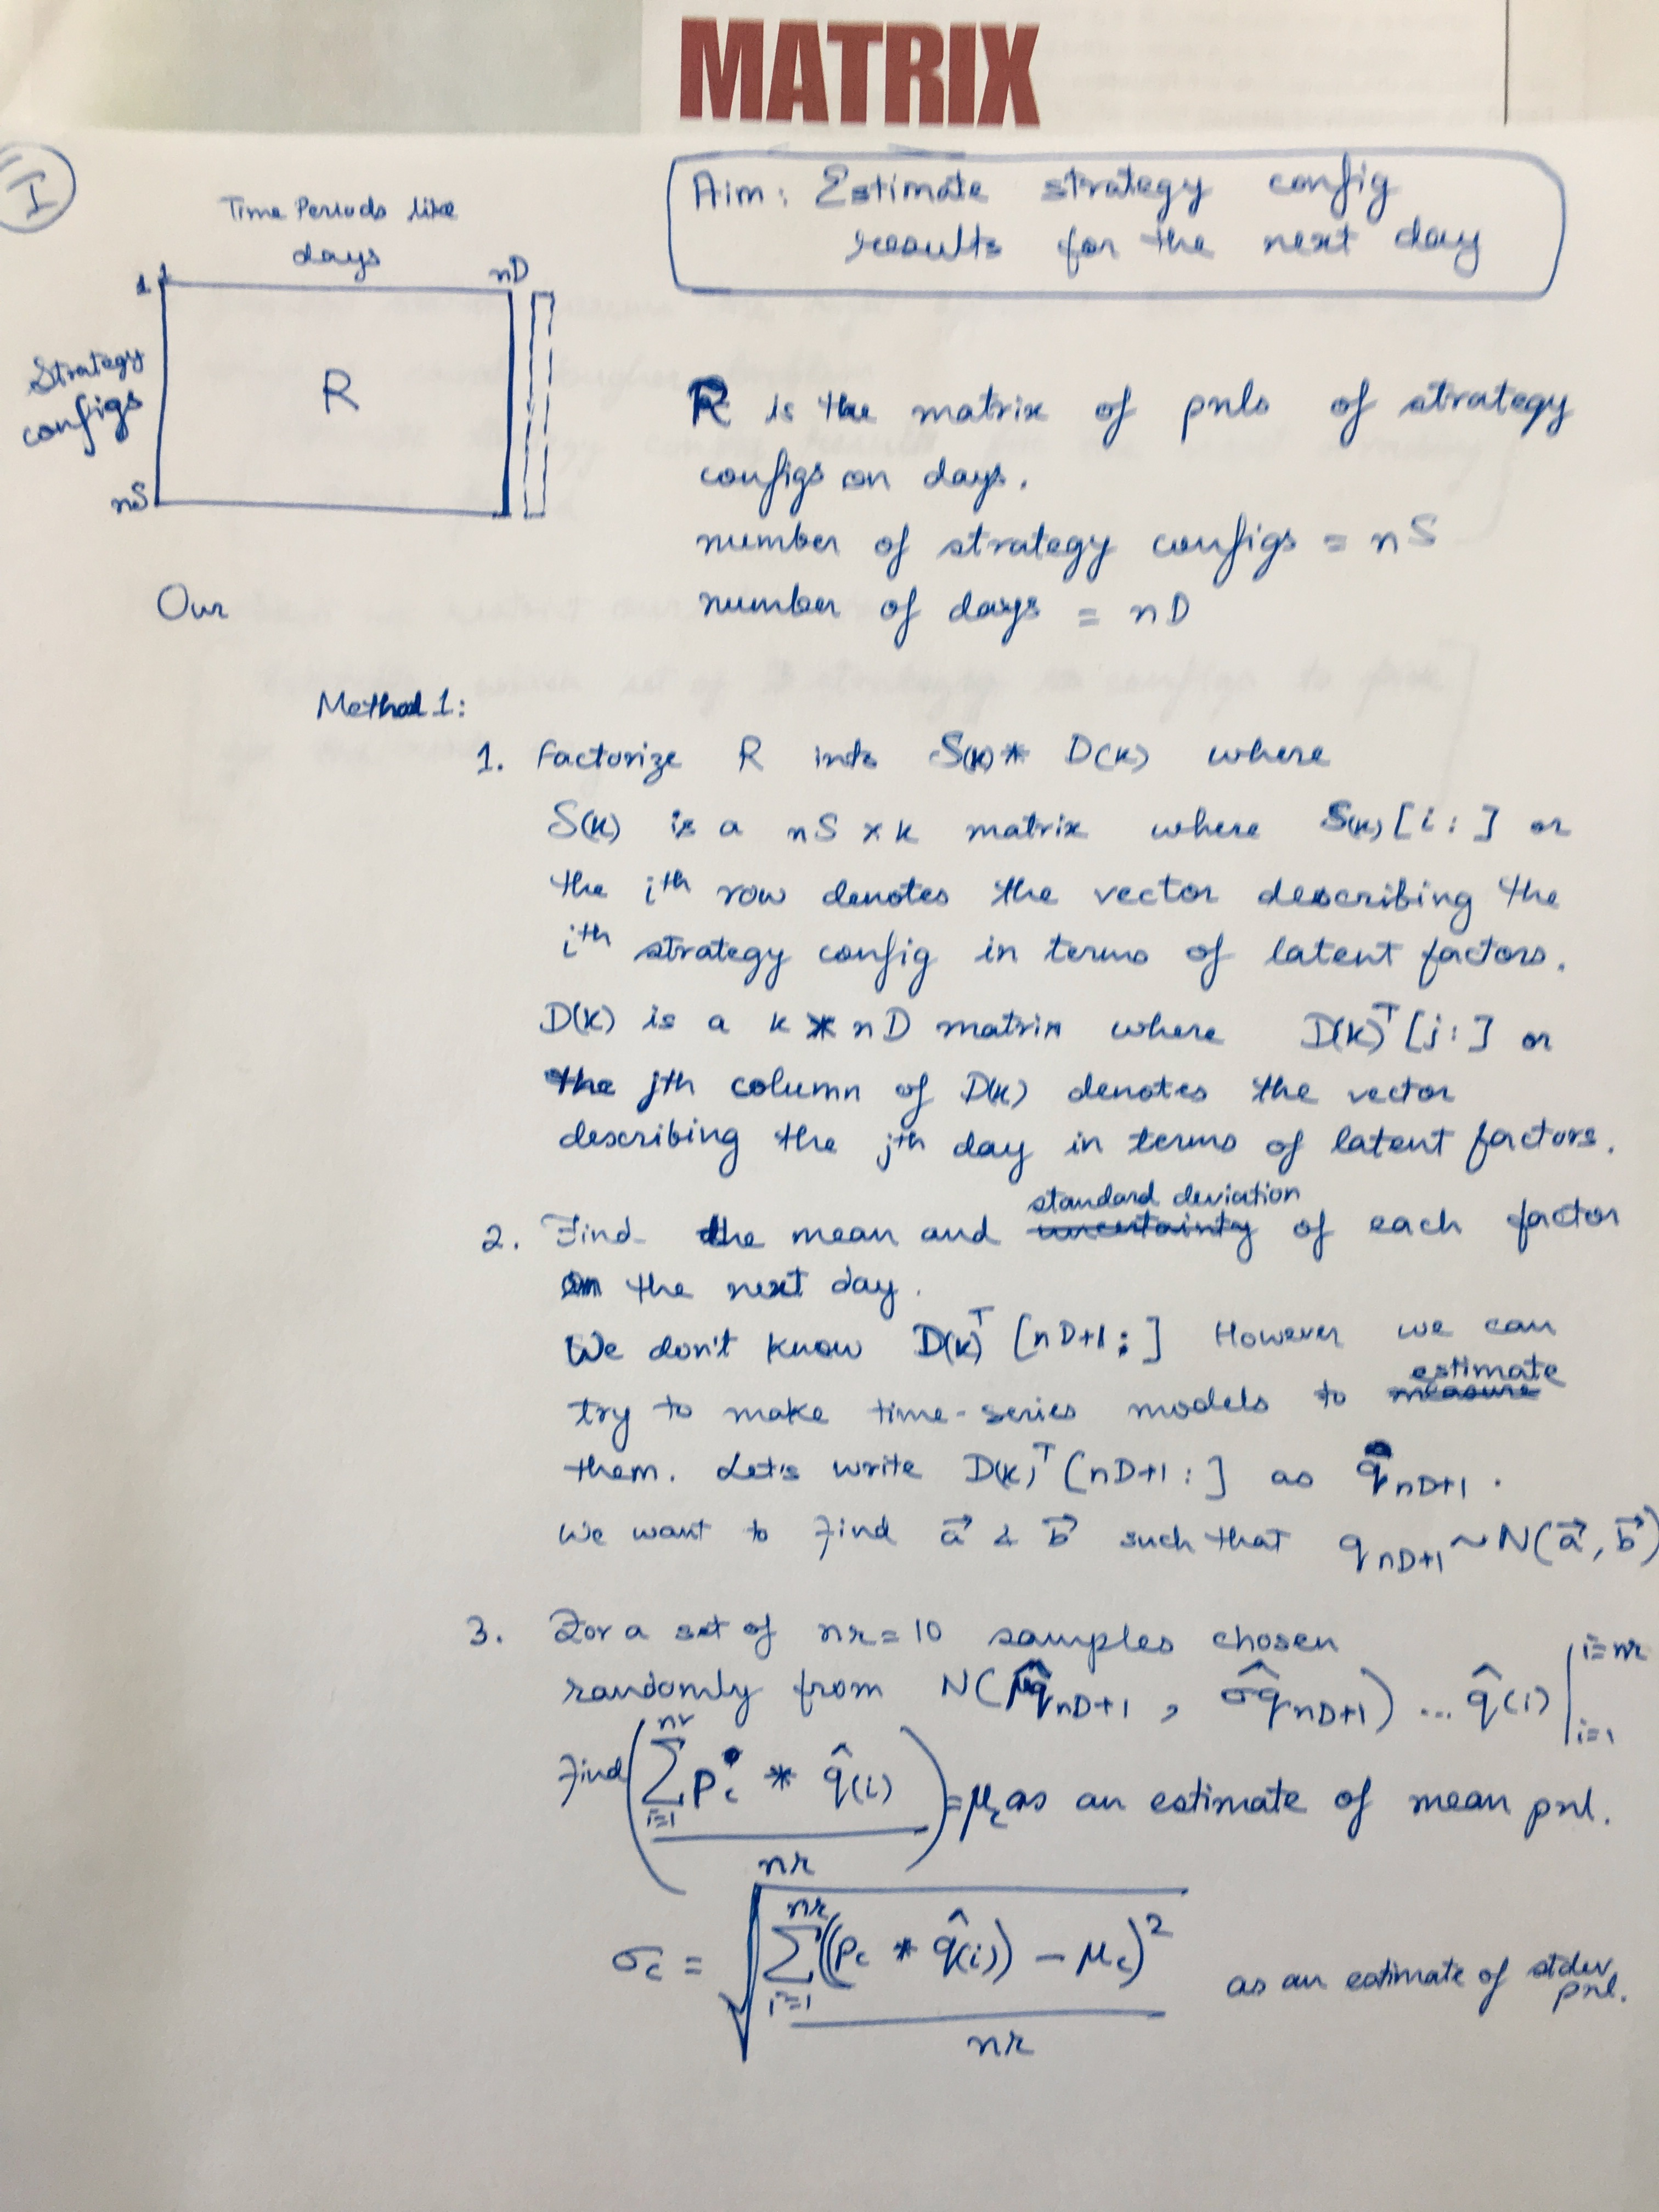
\includegraphics[scale=0.05]{estimate_strategy_config_results_for_next_day_using_collaborative_filtering.jpg}

		
		
		\caption{estimate strategy config results for next day using collaborative filtering}
		\label{fig:estimate strategy config results for next day using collaborative filtering}
		
	\end{figure}
\end{centering}

Figure
\ref{fig:estimate_strategy_config_results_for_next_day_using_collaborative_filtering.jpg}
is just a work in progess idea towards cleaning up this document.

\begin{centering}
	\begin{figure}
		
		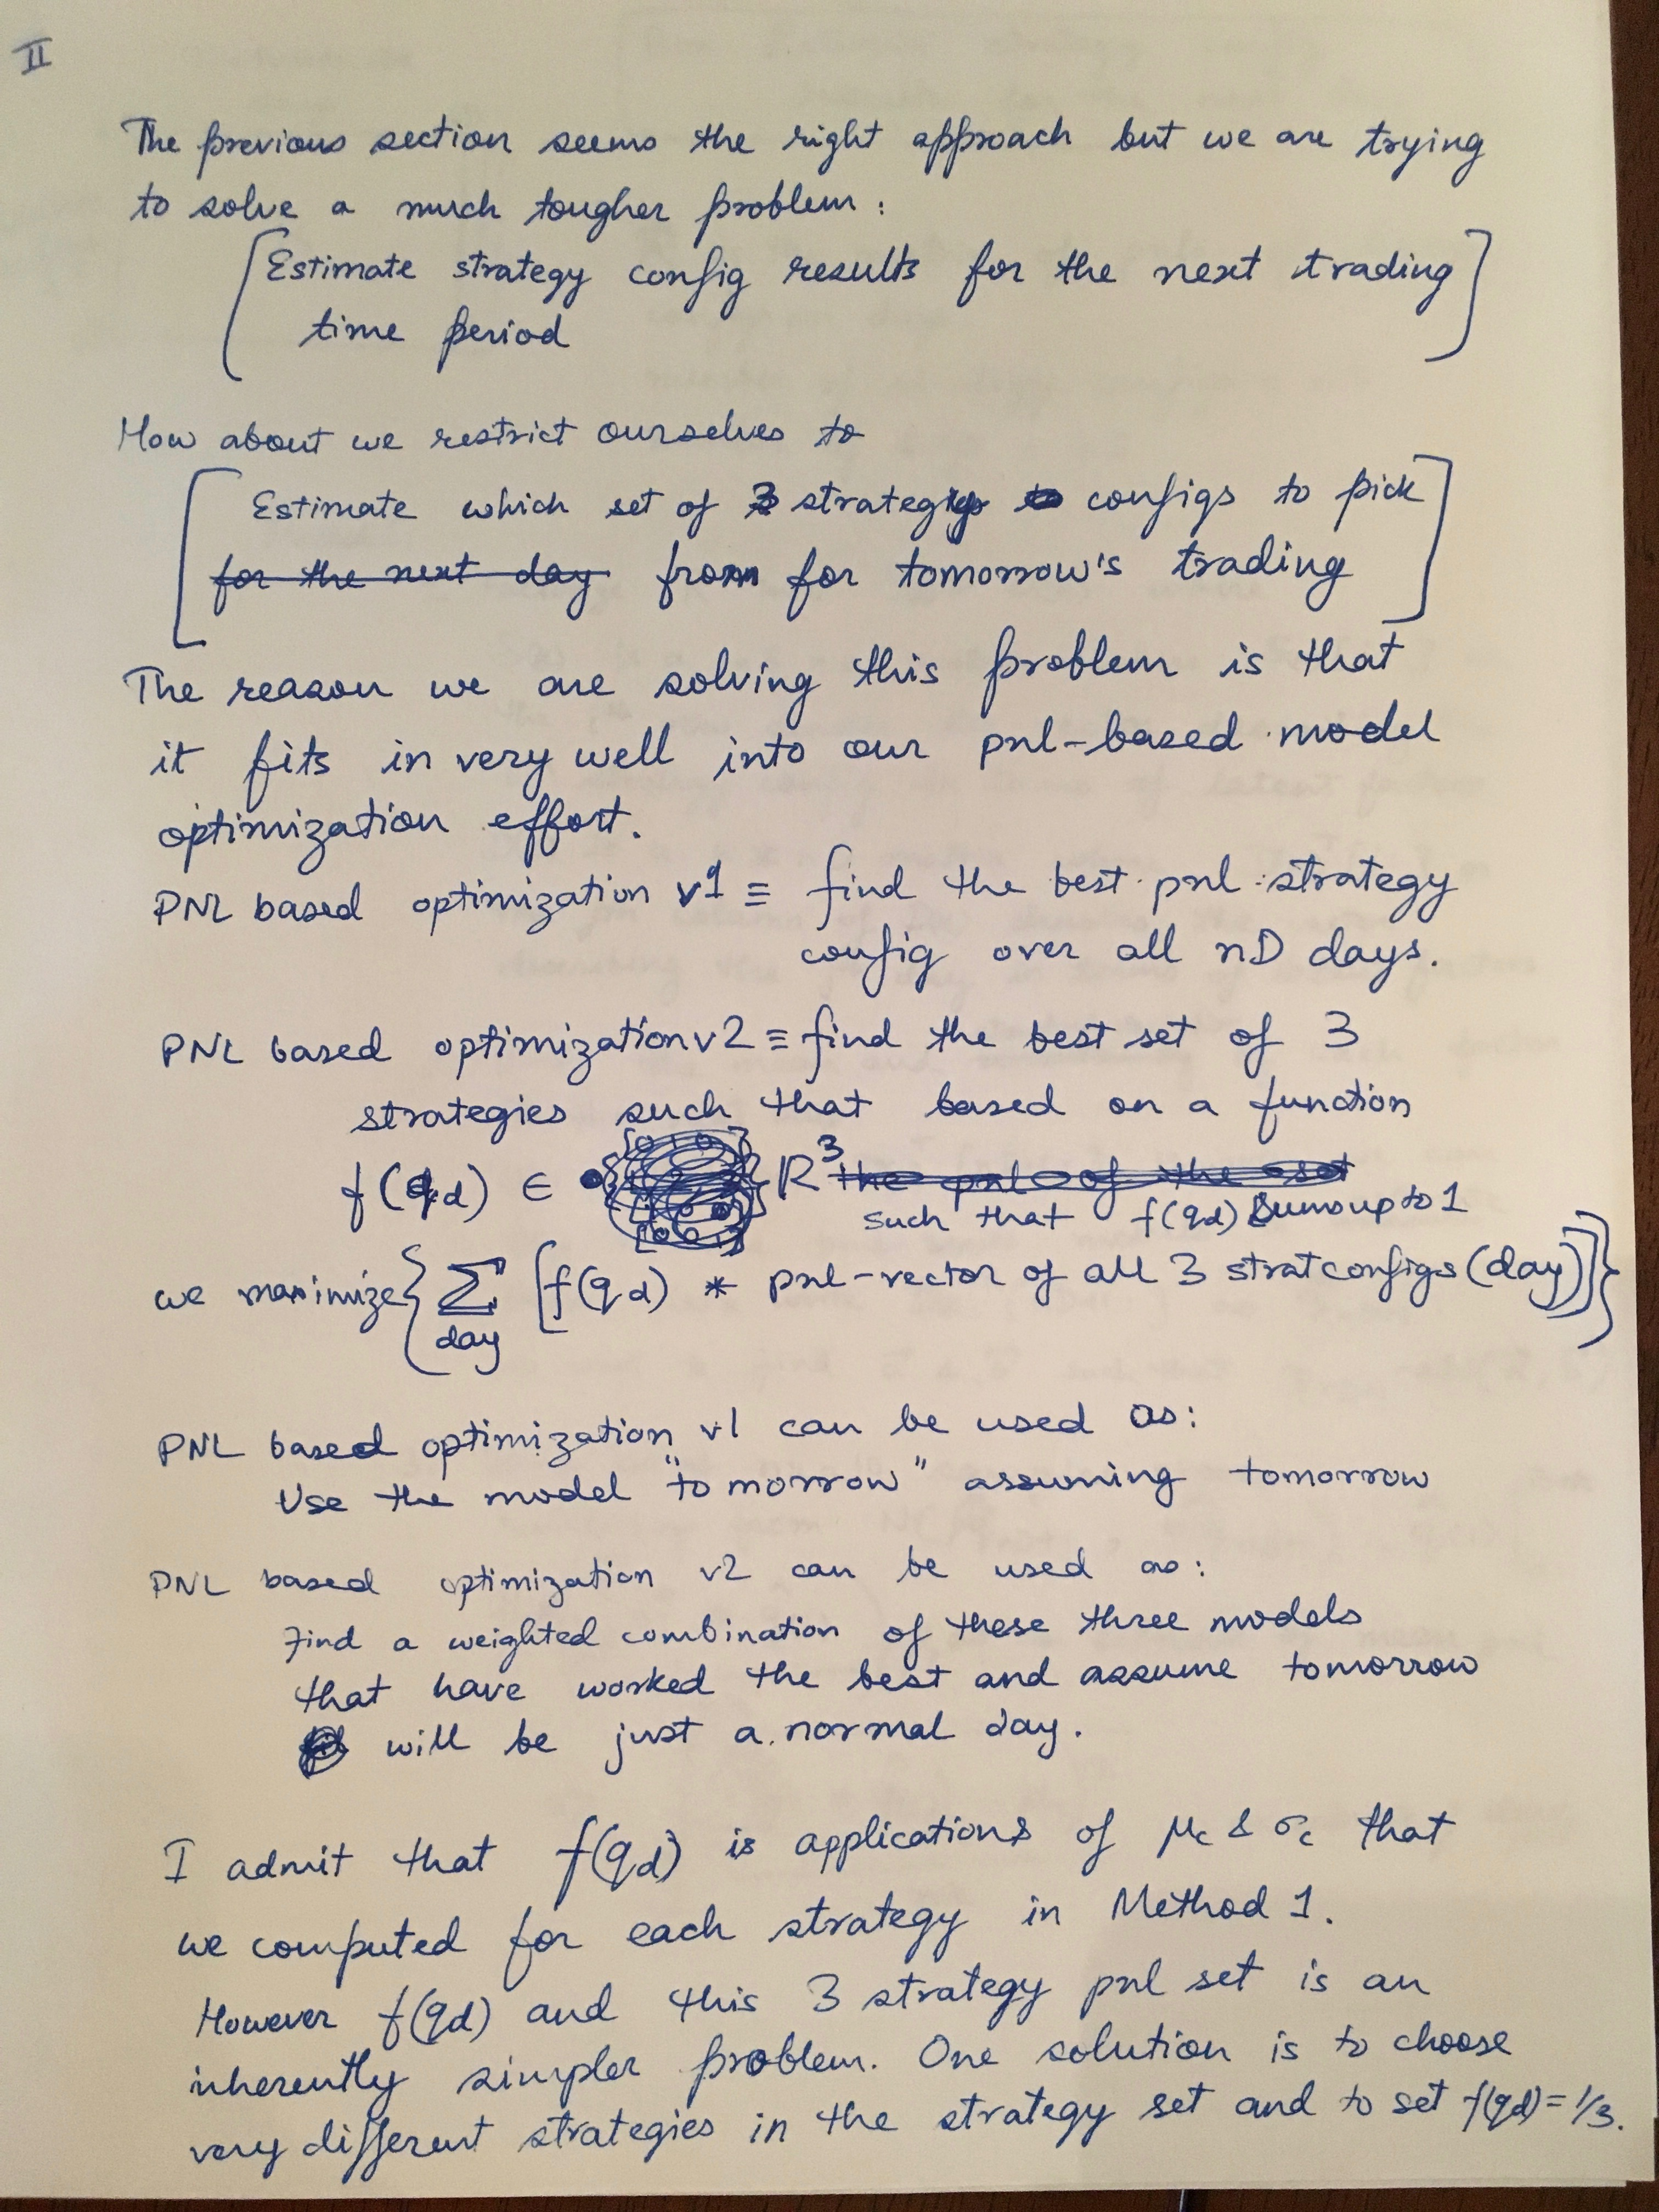
\includegraphics[scale=0.05]{pnl_based_modeling_to_find_a_small_set.jpg}
		
		\caption{pnl based modeling to find a small set}
		\label{fig:pnl based modeling to find a small set}
		
	\end{figure}
\end{centering}

Figure
\ref{fig:pnl based modeling to find a small set}
is just a work in progess idea towards cleaning up this document.

Matrix factorization models maps both strategies and trading days
to a joint latent factor space of dimensionality $k$, such that
strategy-day interactions are modeled as inner products in
that space. Accordingly each strategy config $i$ is associated with a
vector $q_i \in R^k$, and each trading day $d$ is associated with a
vector $p_{d} \in R^k$. For a given strategy $i$, the elements of
$q_i$ measure the extent to which the strategy possesses those
factors, positive or negative. For a given day $d$, the elements of
$p_{d}$ measures factors that describe the day in a way that have a
direct bearing on strategies performance on that day. The resulting
dot product $q_i^T p_{d}$ captures the profitability of strategy $i$
on the day $d$.

\subsection{Robust categorization of trading strategies and dates}
\label{subsec:robust-collaborative-filtering}
To learn the factor vectors $p_{tp}$ and $q_i$, the system minimizes the regularized squared error:
$\sum\limits_{u,i \in \kappa} (r_{ui} - q_i^T*p_{tp})^2 + \lambda(||q_i||^2 = ||p_{tp}||^2)$
Here $\kappa$ is the set of (u,tp) pairs for which $r_{ui}$ is the training set.

We can cluster strategies in this k-dimensional space into
the specified number of clusters, $N_S$. Then we can take either the cluster
centroid or the average of the models in the cluster as a model for
that cluster. This way we would be able to find a set of $N_S$
strategies and models that are both far apart from each other in terms of PnL and also
describe the complete set of trading days. This addresses a
fundamental problem we are facing. We have too many strategies that
are similar. Hence when we try to make a walkforward config based on
choosing between them, it is very hard to really find separability
between them. 

\subsection{Assumptions}
\label{subsec:assumptions}
I am not sure but my hunch is that to use collaborative filtering
method, we might have to make some
changes in terms of converting PnLs to a positive number. 

The assumption in this method is that averaging
models yields a model with expected PnL roughly equal to the average
of the profits of the models we are averaging. This is a strong
assumption. Let's look at one way to circumvent that assumption.\\
Here we can cluster the matrix describing trading days $T$, into $N_S$
clusters. We can then optimize strategies only on the dates in one
cluster and even within the cluster we can assign a lower weight to a trading
date that is far from the cluster centroid. The problems with this
approach would be a greater chance of overfitting since we are
directly optimizing PnL. I would lean more towards the first approach
of averaging models. It appears more robust to me.

\subsection{How to find a good model today given an optimal set}
\label{subsec:daily-retraining}

\subsection{Looking at model selection as a recommender system}
\label{subsec:intuition-recommender}
While working on section \ref{subsec:daily-retraining}, we realized
the similarities between the probem of movie recommendation and
trading strategy selection. We will write more on this philosophical
section when we are high, however I cannot overestimate the need to
look at a problem in the correct perspective. As Alfred Lansing would
say ``That is the right question''.

\section{Computational considerations and algorithmic optimizations}
\label{need-for-speed}
\todo[inline]{We will talk about all the implementation challenges we faced in pnl
space optimization.}  

\bibliographystyle{alpha}
\bibliography{refs}
\newpage
\section{Disclosures \label{disclosures} }
All investments carry risk. This material is for informational purposes only. The factual information set forth herein has been obtained or derived from sources believed to be reliable but it is not necessarily all-inclusive and is not guaranteed as to its accuracy and is not to be regarded as a representation or warranty, express or implied, as to the information’s accuracy or completeness, nor should the attached information serve as the basis of any investment decision. Past performance is not indicative of future performance. Please visit our website \url{https://www.qplum.co/privacy-terms#disclaimer} for full disclaimer and terms of use.\\
This document is intended exclusively for the use of the person to whom it has been delivered and it is not to be reproduced or redistributed to any other person.

\end{document}
